\documentclass[12pt]{article}
\usepackage[utf8]{inputenc}
\usepackage{float}
\usepackage{amsmath}
\usepackage[tableaux]{prooftrees}
\usepackage{indentfirst}
\usepackage{amsfonts}
\usepackage{tikz}
\usepackage{qtree}
\usepackage[hmargin=3cm,vmargin=6.0cm]{geometry}
\renewcommand*\linenumberstyle[1]{(#1)}
\topmargin=-2cm
\addtolength{\textheight}{6.5cm}
\addtolength{\textwidth}{2.0cm}
\setlength{\oddsidemargin}{0.0cm}
\setlength{\evensidemargin}{0.0cm}


\begin{document}

\section*{Student Information}

Name: Kaan Karaçanta \\

ID: 2448546 \\



\section*{Part 1}

% For an input with 4 elements, what would be the matrix that does the inversion operation?
\subsection*{\text{a)}}

$ 2 |\psi \rangle \langle \psi | - I $ where $ |\psi \rangle = \frac{1}{2} \begin{bmatrix} 1 \\ 1 \\ 1 \\ 1 \end{bmatrix} $ and $ I $ is the identity matrix, and the inversion operation matrix is the following:
\[ \frac{1}{2} \begin{bmatrix} -1 & 1 & 1 & 1 \\ 1 & -1 & 1 & 1 \\ 1 & 1 & -1 & 1 \\ 1 & 1 & 1 & -1 \end{bmatrix} \]

% Consider the matrix you defined in part a. Apply that matrix on the input [15, 23, 18, 32]. What
% do you get? What would you get if you apply it again? Briefly explain the result.
\subsection*{\text{b)}}

To apply the matrix on the input, we need to multiply them.  

\[ \frac{1}{2} \begin{bmatrix} -1 & 1 & 1 & 1 \\ 1 & -1 & 1 & 1 \\ 1 & 1 & -1 & 1 \\ 1 & 1 & 1 & -1 \end{bmatrix} \begin{bmatrix} 15 \\ 23 \\ 18 \\ 32 \end{bmatrix} = \frac{1}{2} \begin{bmatrix} 58 \\ 42 \\ 52 \\ 24 \end{bmatrix} = \begin{bmatrix} 29 \\ 21 \\ 26 \\ 12 \end{bmatrix} \]

Then, when we multiply the matrix again with the result, we get the following:

\[ \frac{1}{2} \begin{bmatrix} -1 & 1 & 1 & 1 \\ 1 & -1 & 1 & 1 \\ 1 & 1 & -1 & 1 \\ 1 & 1 & 1 & -1 \end{bmatrix} \begin{bmatrix} 29 \\ 21 \\ 26 \\ 12 \end{bmatrix} = \frac{1}{2} \begin{bmatrix} 30 \\ 46 \\ 36 \\ 64 \end{bmatrix} = \begin{bmatrix} 15 \\ 23 \\ 18 \\ 32 \end{bmatrix} \]

As it can be seen, we get the initial input again. This is because the matrix is the inversion operation matrix, inverts the inputs around their means, and when we apply it twice, it is the same as not applying it at all.

\newpage

% In the attached file you will find a Jupyter notebook based on the IBM Quantum Learning’s Grover
% algorithm (here). Note that we made slight modifications to make it runnable.
\subsection*{\text{c)}}

My student id is 2448546 and its sum 33 is $ 100001 $ in binary. Hence, the oracle function is the following:

\begin{figure}[H]
    \centering
    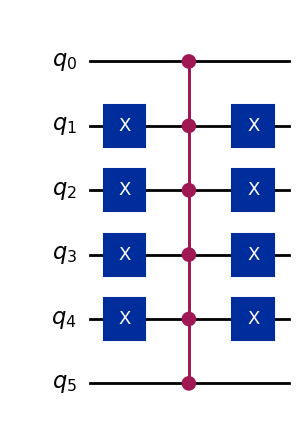
\includegraphics[width=0.3\textwidth]{oracle.png}
    \caption{Oracle function}
\end{figure}

The Grover operator is the following:

\begin{figure}[H]
    \centering
    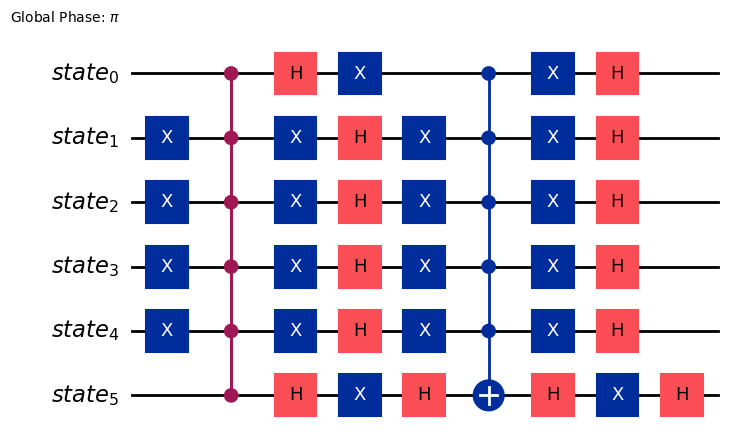
\includegraphics[width=0.8\textwidth]{groverOp.png}
    \caption{Grover operator}
\end{figure}

\newpage

The final circuit is the following:

\begin{figure}[H]
    \centering
    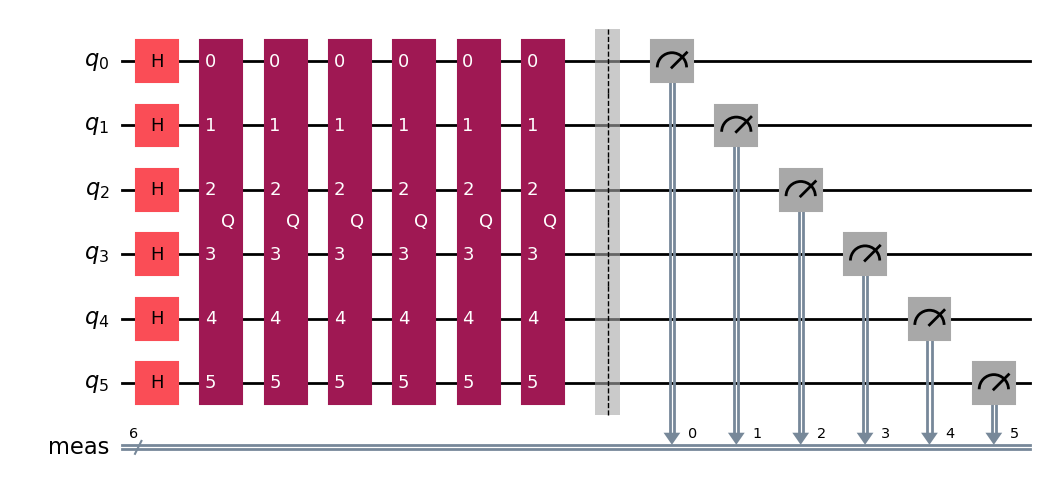
\includegraphics[width=0.9\textwidth]{groverCirc.png}
    \caption{Final circuit}
\end{figure}

The result of the circuit is the following:

\begin{figure}[H]
    \centering
    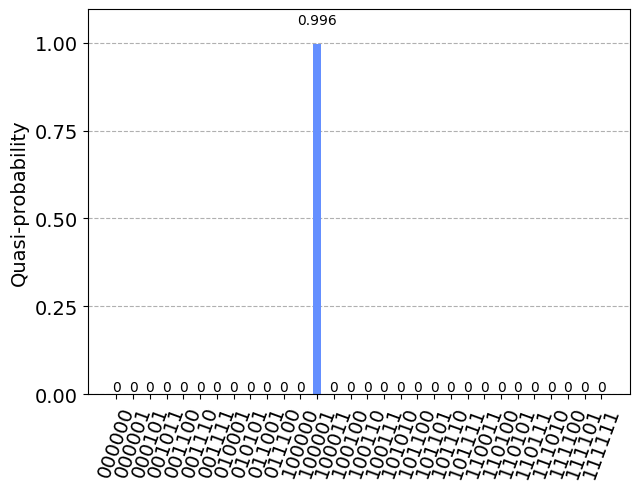
\includegraphics[width=0.7\textwidth]{distribution.png}
    \caption{Final plot of the distributions}
\end{figure}

\newpage

The plot shows a single dominant peak, with a quasi-probability very close to 1 (labeled as 0.996 on the plot), which is significantly higher than for any other state. This peak corresponds to the state that Grover's algorithm has identified as the solution to the search problem.

As a search algorithm, Grover's algorithm works by repeatedly applying an oracle that inverts the phase of the solution state, and then a diffusion operator that amplifies the amplitude of the state(s) with a negative phase. The result is that the amplitude (and thus the probability upon measurement) of the correct state becomes much larger than that of the incorrect states.


\subsection*{\text{d)}}

The original number of iterations was set to be optimal, which was calculated like this  $ \lfloor \frac{\pi}{4} * \sqrt{\frac{2^{n}}{m}} \rfloor $, where $ n $ is the number of qubits and $ m $ is the number of marked states. In this case, $ n = 6 $ and $ m = 1 $, so the number of iterations is $ \frac{\pi}{4} * \sqrt{\frac{2^{6}}{1}} = 6.2832 $, so it was taken as 6. First, I tried to run the circuit with 8 iterations, and the result is the following:

\begin{figure}[H]
    \centering
    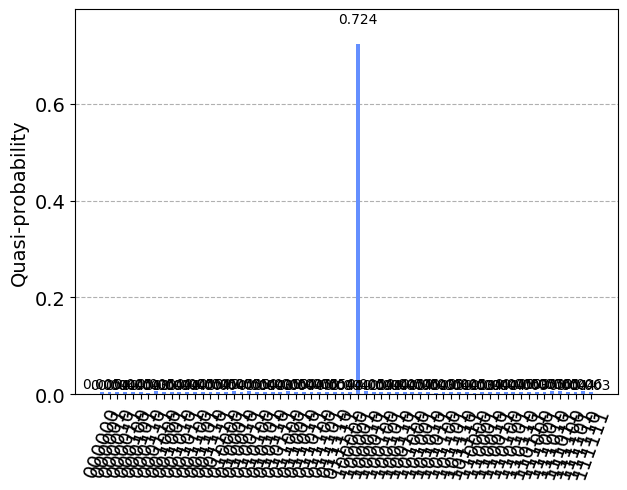
\includegraphics[width=0.7\textwidth]{distribution8.png}
    \caption{Plot of the distributions with 8 iterations}
\end{figure}

Although, there are many points on the x axis now, so it is checking some other states, and the peak point is lower than the optimal number of iterations, the result is clearly visible. The peak is still the same with the quasi-probability 0.724.

\newpage

Then, I tried to run the circuit with 10 iterations, and the result is the following:

\begin{figure}[H]
    \centering
    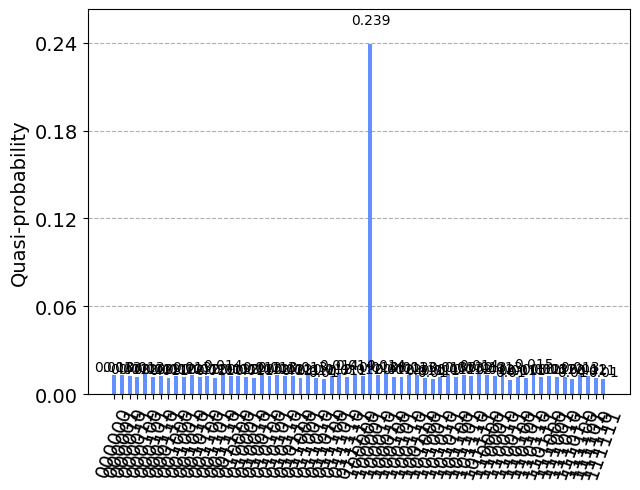
\includegraphics[width=0.6\textwidth]{distribution10.png}
    \caption{Plot of the distributions with 10 iterations}
\end{figure}

The peak is much more lower than the one with the optimal number of iterations, and the probability of it is 0.239. Besides, now other points on the x axis are have higher quasi-probabilities than the previous ones. However, they are still much lower than 0.239, so it is still working.

Finally, when I tried to run the circuit with 12 iterations, the result is the following:

\begin{figure}[H]
    \centering
    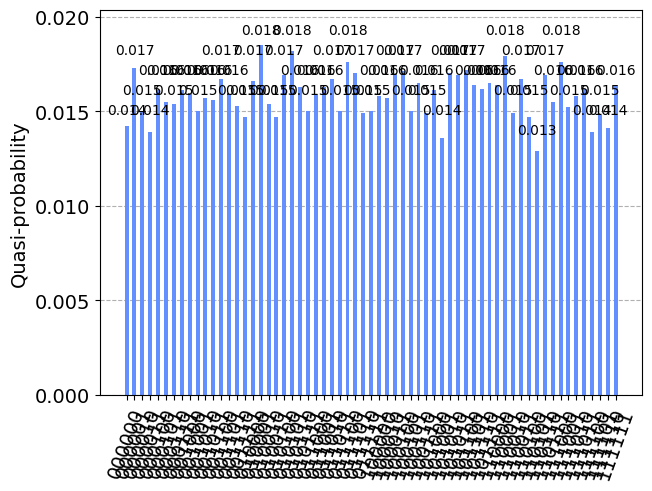
\includegraphics[width=0.65\textwidth]{distribution12.png}
    \caption{Plot of the distributions with 12 iterations}
\end{figure}

From this plot, nothing much can be understood, the probabilities are very close to each other and not even visible in the plot. Thus, the algorithm is not working with 12 iterations. 

The reason why such a thing happened is that Grover's algorithm iteration is rotation of any state in the circle over an angle 2$\Theta$ where $\Theta$ is $ arcsin(\frac{1}{\sqrt{n}}) $,  and the algorithm works on (2k+1)$\Theta$ where k is an integer. So, the algorithm works with 6 iterations, but not with 12 iterations. 
Also, I tried further, and it is starting to work again when I increased the number of iterations up to 18, which is the same as 6, then again until 24, the success rate is decreasing, and with 24, it is not working as the case for 12. This is sometimes referred to as "overshooting" the target state.

\section*{Part 2}


\subsection*{\text{a)}}

\begin{enumerate}
    \item True
    \item False. QFT circuit contains mixture of Hadamard and phase gates, but not CNOT gates.
    \item False. The phase gate $R_k$ used in QFT is $ R_k = \begin{bmatrix} 1 & 0 \\ 0 & e^{\frac{2 \pi i}{2^k}} \end{bmatrix} $. 
    \item True
    \item False. Quantum phase estimation is a crucial part of Shor's factorization algorithm as it is used to find the order of an element which is key to factorization.
\end{enumerate}


\subsection*{\text{b)}}

Here is the circuit for the QFT with my id "100001" in binary:

\begin{figure}[H]
    \centering
    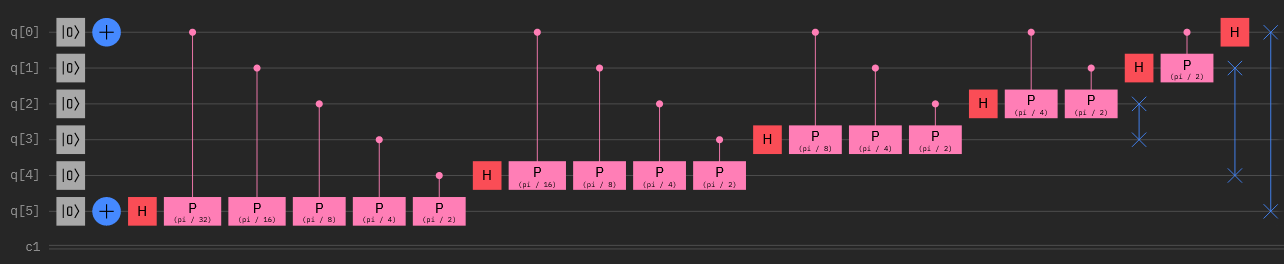
\includegraphics[width=0.95\textwidth]{qft_circ.png}
    \caption{QFT circuit}
\end{figure}

\newpage

Here is the plot of the results, not quite readable:

\begin{figure}[H]
    \centering
    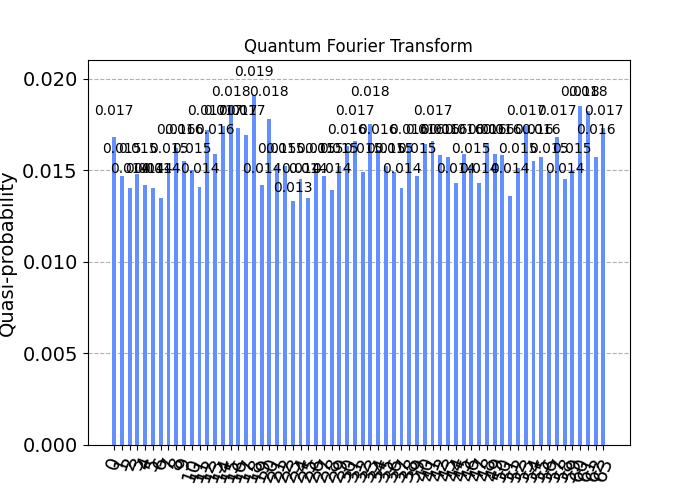
\includegraphics[width=0.65\textwidth]{qft_dist.png}
    \caption{Plot of the results}
\end{figure}

As it is not readable, I printed the results as a table:

\begin{figure}[H]
    \centering
    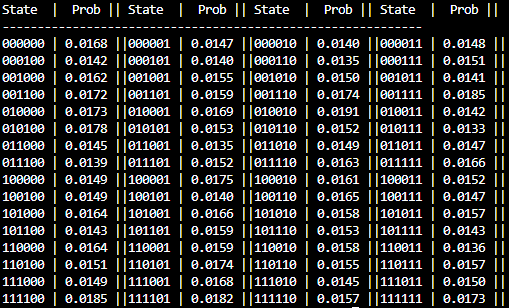
\includegraphics[width=0.7\textwidth]{qft_table.png}
    \caption{Table of the results}
\end{figure}

With these results, in summary, QFT has taken the inital state $ |100001\rangle $, and transformed it into a complex superposition of all possible states, with amplitudes that reflect the Fourier transform of the initial state. This non-uniform distribution is a direct consequence of the input state and the QFT operation.

\end{document}
